\documentclass[10.5pt,scale=1.0,t,aspectratio=169,hyperref={pdfpagelabels=false}]{beamer}
%\usepackage[paperwidth=13.33in, paperheight=7.5in,top=.25in, bottom=.25in, left=.25in, right=.25in]{geometry}
%\geometry{papersize={13.33in,7.5in}}

%\usetheme{Dresden}
%\usetheme{Warsaw}

%Other themes
%https://hartwork.org/beamer-theme-matrix/

\usepackage{lipsum}
\usepackage{color}

\usepackage{amsfonts}
\usepackage{amsmath,mathtools}
\usepackage{mathrsfs}
\usepackage{array}
\usepackage{algorithm}
\usepackage{hyperref}
\usepackage[spanish,es-nodecimaldot]{babel}
\usepackage[utf8]{inputenc}
%\usepackage{intcalc}
\usepackage{graphicx}
\usepackage{multicol}
%\usepackage{authblk}
\usepackage{multirow}
\usepackage{enumitem}
\usepackage[document]{ragged2e}

\usepackage[absolute,overlay]{textpos}
\textblockorigin{0mm}{0mm} 

\usefonttheme[onlymath]{serif}
%\usepackage{epstopdf}
\usepackage{verbatim}
\usepackage{cite}
%\usepackage[texcoord,grid,gridunit=mm,gridcolor=red!10,subgridcolor=green!10]{eso-pic}




\newenvironment{conditions}[1][where:]
  {#1 \begin{tabular}[t]{>{$}l<{$} @{${}={}$} l}}
  {\end{tabular}\\[\belowdisplayskip]}


\newcolumntype{L}{>{$}l<{$}} % math-mode version of "l" column type


\newcounter{saveenumi}
\newcommand{\seti}{\setcounter{saveenumi}{\value{enumi}}}
\newcommand{\conti}{\setcounter{enumi}{\value{saveenumi}}}

\setbeamertemplate{bibliography item}{\insertbiblabel}


\hypersetup{colorlinks=true,
						linkcolor=blue,
						linktoc=all,				
						citecolor=blue,
						urlcolor=red,
						pdftitle={ELECTRONICA DIGITAL II},
						pdfauthor={Santiago Rúa Pérez},
						pdfcreator={Santiago Rúa Pérez}}


\definecolor{GreenDark}{rgb}{0.0, 0.60, 0.0}
\definecolor{RedDark}{rgb}{183, 0.0, 0.0}
\definecolor{BlueDark}{rgb}{0.0, 0.0, 167}
\definecolor{BlueLight}{rgb}{0.2, 0.451, 0.517}


\graphicspath{{imag/}}

\newcommand{\Ho}{$H_{0}$}
\newcommand{\Ha}{$H_{a}$}
\newcommand{\Nota}{{\bf Nota: }}
\newcolumntype{P}[1]{>{\centering\arraybackslash}p{#1}}
\newcolumntype{M}[1]{>{\centering\arraybackslash}m{#1}}

\newcommand{\less}{<}
\newcommand{\greater}{>}


\setlength{\parindent}{1em}
\setlength{\parskip}{.6em}
\renewcommand{\baselinestretch}{.9}

 
\title{Electrónica Digital II}   
\author{Santiago Rúa Pérez, PhD.} 
\date{\today} 

\setlength{\TPHorizModule}{\textwidth}
\setlength{\TPVertModule}{\textwidth}

\newcommand{\btVFill}{\vskip0pt plus 1filll}


\setbeamertemplate{sidebar right}{}
\setbeamertemplate{footline}
{
	\leavevmode%
	\hbox{%
		\begin{beamercolorbox}[wd=.333333\paperwidth,ht=2.25ex,dp=1ex,center]{author in head/foot}%
			\usebeamerfont{author in head/foot}\insertshortauthor
		\end{beamercolorbox}%
		\begin{beamercolorbox}[wd=.333333\paperwidth,ht=2.25ex,dp=1ex,center]{title in head/foot}%
			\usebeamerfont{title in head/foot}\insertshorttitle
	\end{beamercolorbox}}%
	\vskip0pt%
}
\makeatother

\begin{document}
\justify
\renewcommand{\arraystretch}{2.0}


%%%%%%%%%%%%%%%%%% FRAME %%%%%%%%%%%%%%%%%%%%%%%%%%
\begin{frame}
	\titlepage
\end{frame}
%%%%%%%%%%%%%%%%%%% FRAME %%%%%%%%%%%%%%%%%%%%%%%%%%



%%%%%%%%%%%%%%%%% FRAME %%%%%%%%%%%%%%%%%%%%%%%%%%
\begin{frame}
	\frametitle{Identificación}
	{\bf Datos del curso}
	\begin{itemize}
		\item Asignatura: Electrónica Digital II 
		\item Dias: Martes-Jueves 12-2 pm. Salon 3-218
		\item Créditos: 3
		\item Docente: Santiago Rúa Pérez
		\item Correo: srua@udemedellin.edu.co
	\end{itemize}
\end{frame}
%%%%%%%%%%%%%%%%% FRAME %%%%%%%%%%%%%%%%%%%%%%%%%%

%%%%%%%%%%%%%%%%% FRAME %%%%%%%%%%%%%%%%%%%%%%%%%%
\begin{frame}
	\frametitle{Competencias del curso}
	
	\begin{itemize}
		\justifying
		\item Adquirir habilidades en el uso del lenguaje de programación C para sistemas embebidos.
		\item Manipular, clasificar y desarrollar aplicaciones con los periféricos básicos de un microcontrolador de mediana complejidad.
		\item Distinguir y aplicar diferentes técnicas de comunicación serial usando un microcontrolador.
		\item Desarrollar aplicaciones microcontroladas teniendo en cuenta ciertas restricciones de diseño.
		\item Adoptar buenas prácticas de desarrollo, análisis y depuración de aplicaciones embebidas.
	\end{itemize}
\end{frame}

%%%%%%%%%%%%%%%%% FRAME %%%%%%%%%%%%%%%%%%%%%%%%%%
\begin{frame}
	\frametitle{Compromiso académico}
	
	\begin{columns}
		\column{0.5\linewidth}
			\textcolor{blue}{\large Evaluación del curso - teórico} \\
			Trabajo I: 25\%, 23 de Agosto\\
			Lab 1: 10\%, 30 de Agosto\\ 
			Lab 2: 10\%, 8 de Septiembre\\
			Lab 3: 15\%, 27 de Septiembre\\ 
			Lab 4: 15\%, 20 de Octubre\\
			Trabajo Final: 25\%, 17 de Noviembre\\
			\vspace{0.5cm}
			
			\textcolor{blue}{\large Registro de notas} \\
			Registro 75\%: 1 de noviembre. \\
			Registro 100\%: 18 de noviembre. \\
			
		\column{0.5\linewidth}
			\textbf{Con 6 clases o 12 horas directas se cancela el curso. }
	\end{columns}
\end{frame}
%%%%%%%%%%%%%%%%% FRAME %%%%%%%%%%%%%%%%%%%%%%%%%%
\begin{frame}
	\frametitle{Compromiso académico}
	\textcolor{blue}{\large Cronograma}
	\vspace{-0.2in} 		
	\begin{figure}
		\centering
		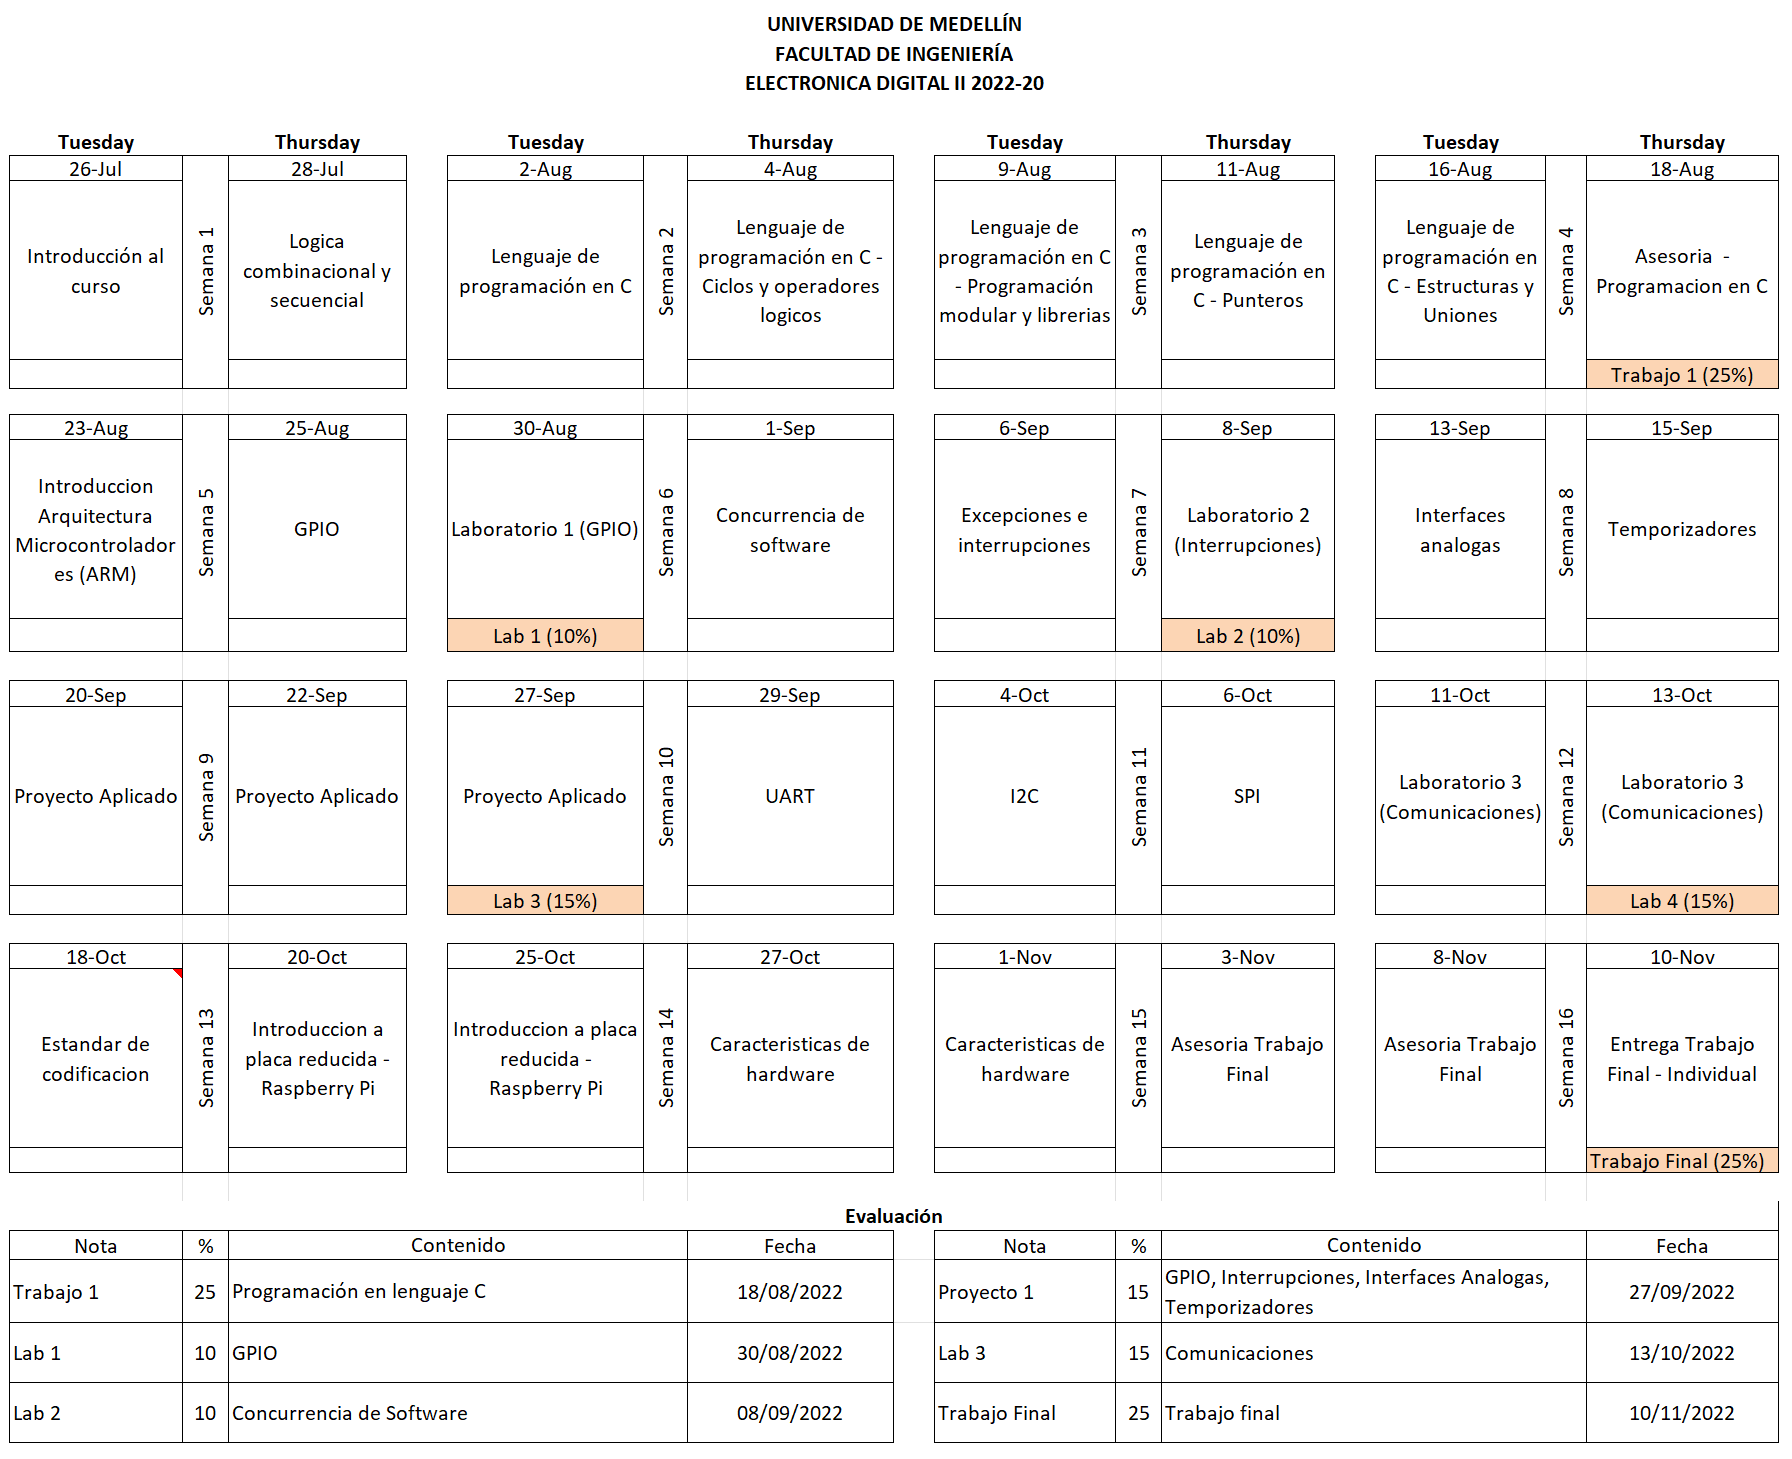
\includegraphics[width=10cm,height=7cm]{CronogramaElectronicaDigitalII}
	\end{figure}
\end{frame}
%%%%%%%%%%%%%%%%% FRAME %%%%%%%%%%%%%%%%%%%%%%%%%%
\begin{frame}
	\frametitle{Software y Hardware}
	\textcolor{blue}{Software}
	\begin{itemize}
		\item MCUExpresso
		\item Compilador de C (VSCode)
		\item Arduino 
	\end{itemize}
	
	\textcolor{blue}{Hardware}
	\begin{itemize}
		\item Kit de Laboratorio por estudiante
	\end{itemize}
\end{frame}

%%%%%%%%%%%%%%%%% FRAME %%%%%%%%%%%%%%%%%%%%%%%%%%
\begin{frame}
	\frametitle{Kit de Laboratorio}
	\begin{figure}
		\centering
		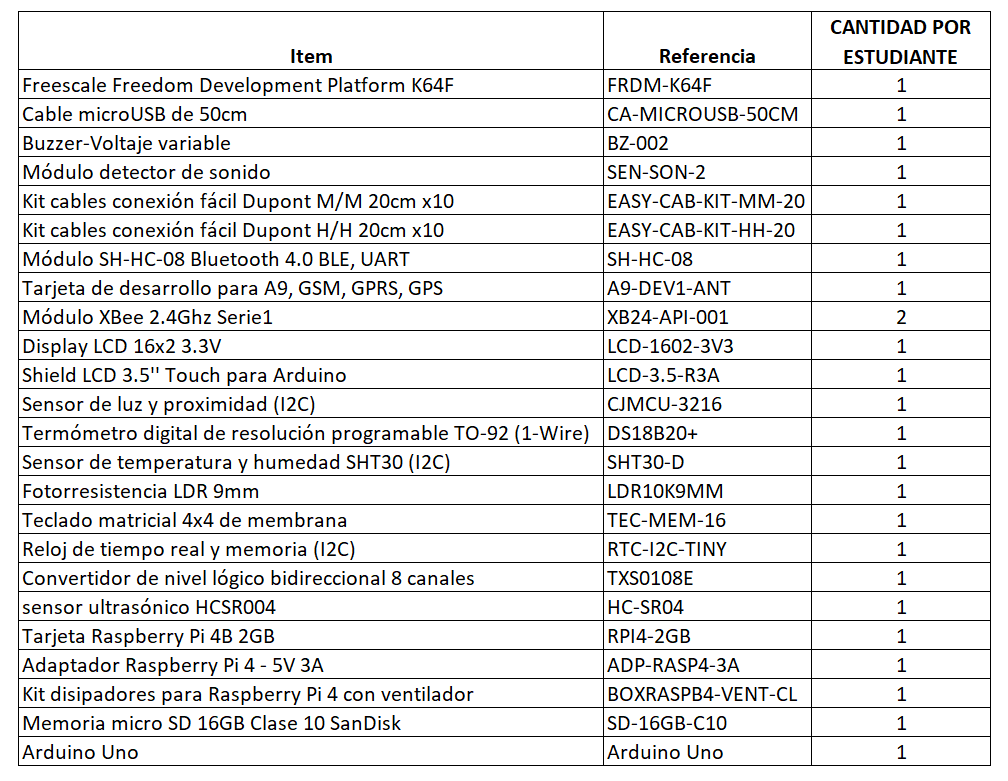
\includegraphics[scale=0.5]{KitLabEmbebidos}
	\end{figure}
\end{frame}
%%%%%%%%%%%%%%%%% FRAME %%%%%%%%%%%%%%%%%%%%%%%%%%
\begin{frame}
	\frametitle{Introducción a los sistemas embebidos}
	\begin{itemize}
		\item \textcolor{BlueLight}{Qué es un sistema embebido?} 
		\begin{itemize}
			\item Aplicaciones específicas de los sistemas de cómputo
			\item Se utilizan en sistema mas complejos.
		\end{itemize}
		\item \textcolor{BlueLight}{Porque usar un computador en un sistema complejo?}
		\begin{itemize}
			\item Mejor desempeño.
			\item Mas funciones y características.
			\item Bajo costo.
			\item Mayor dependencia.
		\end{itemize}
		\item \textcolor{BlueLight}{Economía}
		\begin{itemize}
			\item Microcontroladores se produce en alto volúmenes. 
			\item Costo no recurrente dominado por el desarrollo de software
		\end{itemize}
		\item\textcolor{BlueLight}{Red}
		\begin{itemize}
			\item A menudo, el sistema integrado utilizará varios procesadores que se comunican a través de una red para reducir los costos de piezas y ensamblaje y mejorar la confiabilidad.
		\end{itemize}
	\end{itemize}
\end{frame}
%%%%%%%%%%%%%%%%% FRAME %%%%%%%%%%%%%%%%%%%%%%%%%%
\begin{frame}
	\frametitle{Opciones para construir Sistemas Embebidos}
	\begin{figure}
		\centering
		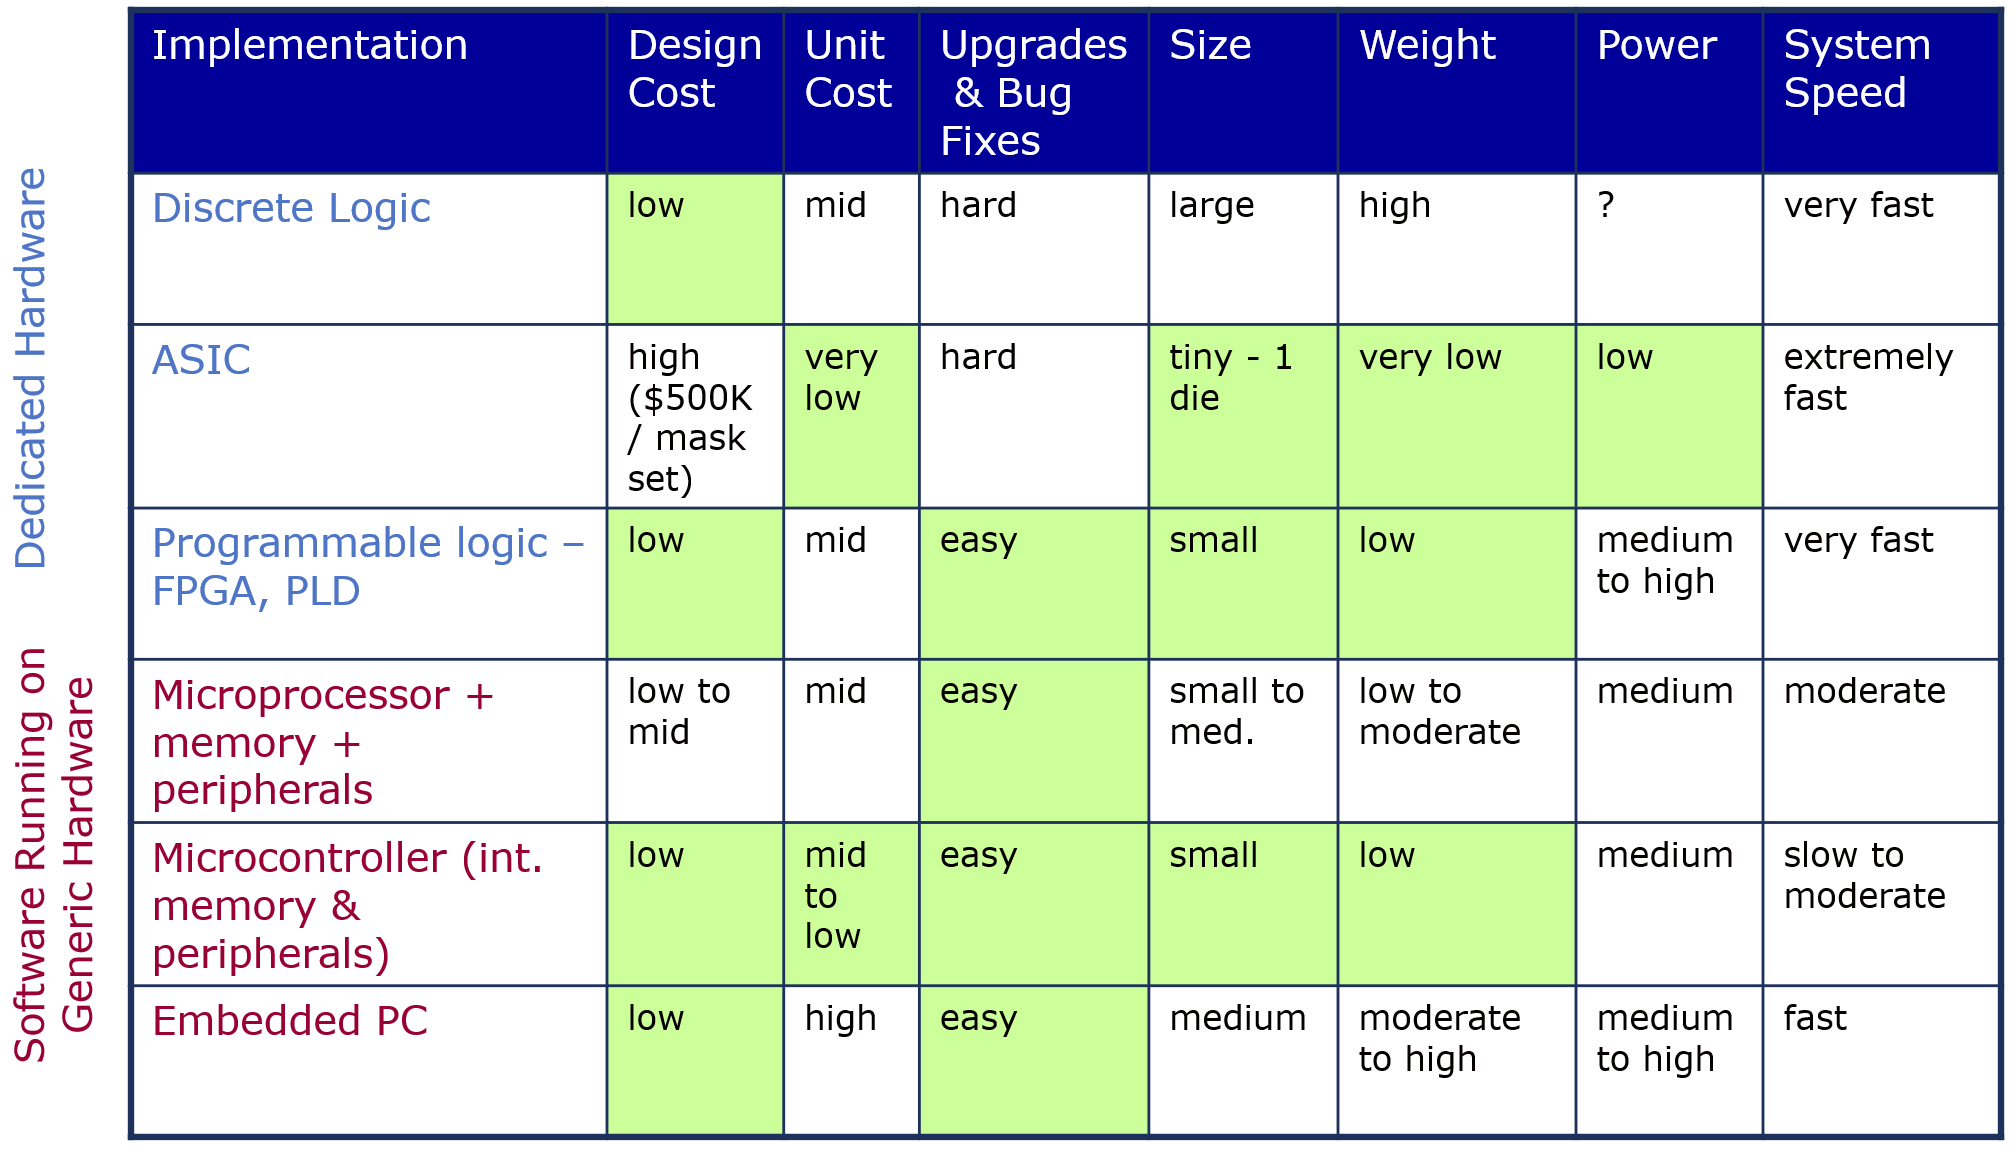
\includegraphics[scale=0.35]{BuildEmbbededSystems}
	\end{figure}
\end{frame}
%%%%%%%%%%%%%%%%% FRAME %%%%%%%%%%%%%%%%%%%%%%%%%%
\begin{frame}
	\frametitle{Ejemplo sistema embebido: PC de bicicleta}
	\begin{columns}
		\column{0.5\linewidth}
		\begin{itemize}
			\item \textcolor{BlueLight}{Funciones}
			\begin{itemize}
				\item Medir velocidad y distancia.
				\item Calcular quema de calorias.
			\end{itemize}
			\item \textcolor{BlueLight}{Restricciones}
			\begin{itemize}
				\item Tamaño.
				\item Costo.
				\item Potencia y consumo de energía.
				\item Peso.
			\end{itemize}
			\item \textcolor{BlueLight}{Entradas}
			\begin{itemize}
				\item Sensor de rotación de la rueda.
				\item Teclado de entrada para modos.
			\end{itemize}
			\item \textcolor{BlueLight}{Salida}
			\begin{itemize}
				\item Pantalla de cristal líquido.
			\end{itemize}
			\item \textcolor{BlueLight}{MCU de bajo rendimiento}
			\begin{itemize}
				\item 8-bits, 10 MIPS.
			\end{itemize}
		\end{itemize}
		
		\column{0.5\linewidth}
		\begin{figure}
			\centering
			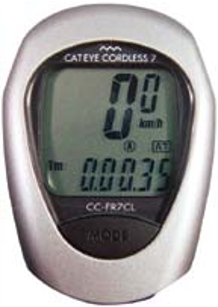
\includegraphics[scale=0.7]{BikePC}
		\end{figure}		
	\end{columns}
\end{frame}
%%%%%%%%%%%%%%%%% FRAME %%%%%%%%%%%%%%%%%%%%%%%%%%
\begin{frame}
	\frametitle{Ejemplo: Unidad de control motor de gasolina}
	\begin{columns}
		\column{0.5\linewidth}
		\begin{itemize}
			\item \textcolor{BlueLight}{Funciones}
			\begin{itemize}
				\item Inyección de combustible, toma de aire.
				\item Tiempo de chispa.
				\item Circulación de gases de escape. 
				\item Control electrónico acelerador.
			\end{itemize}
			\item \textcolor{BlueLight}{Restricciones}
			\begin{itemize}
				\item Fiabilidad en entornos hostiles
				\item Costo y peso.
			\end{itemize}
			\item \textcolor{BlueLight}{Muchas entradas y salidas}
			\begin{itemize}
				\item Sensores discretos y actuadores
				\item Interfaz de red en el carro.
			\end{itemize}
			\item \textcolor{BlueLight}{MCU de alto desempeño}
			\begin{itemize}
				\item 32-bits, 3 MB flash, 150-300 MHz.
			\end{itemize}
		\end{itemize}
		
		\column{0.55\linewidth}
		\begin{figure}
			\centering
			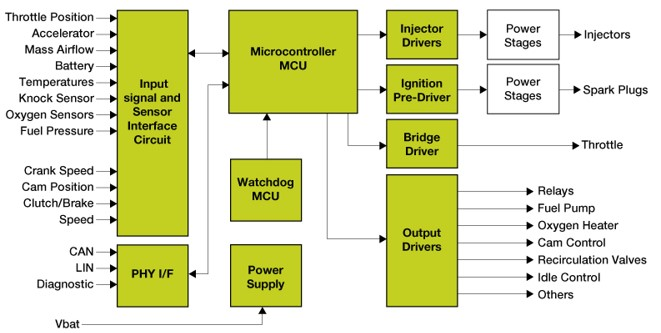
\includegraphics[scale=0.45]{ControlUnitEngine}
		\end{figure}		
	\end{columns}
\end{frame}
%%%%%%%%%%%%%%%%% FRAME %%%%%%%%%%%%%%%%%%%%%%%%%%
\begin{frame}
	\frametitle{Beneficios de los sistemas embebidos}
	\begin{itemize}
	\item \textcolor{BlueLight}{Gran desempeño y eficiencia} 
		\begin{itemize}
			\item El software permite proporcionar un control sofisticado.
		\end{itemize}
	\item \textcolor{BlueLight}{Bajo costo} 
		\begin{itemize}
			\item Se pueden utilizar componentes menos costosos.
			\item Reducción de los costes de fabricación.
			\item Costos operativos reducidos.
			\item Reducción de los costes de mantenimiento.
		\end{itemize}
	\item \textcolor{BlueLight}{Mas características} 
		\begin{itemize}
			\item Muchos no son posibles o prácticos con otros enfoques.
		\end{itemize}
	\item \textcolor{BlueLight}{Mejor confiabilidad} 
	\begin{itemize}
		\item Sistema adaptativo que puede compensar fallas.
		\item Mejores diagnósticos para mejorar el tiempo de reparación.
	\end{itemize}
\end{itemize}	
\end{frame}
%%%%%%%%%%%%%%%%% FRAME %%%%%%%%%%%%%%%%%%%%%%%%%%
\begin{frame}
	\frametitle{Funciones de los sistemas embebidos}
	\begin{itemize}
		\item \textcolor{BlueLight}{Sistemas de control en lazo cerrado} 
		\begin{itemize}
			\item Monitoree un proceso, ajuste una salida para mantener el punto de ajuste deseado (temperatura, velocidad, dirección, etc.)
		\end{itemize}
		\item \textcolor{BlueLight}{Secuenciación} 
		\begin{itemize}
			\item Pasar por diferentes etapas según el entorno y el sistema.
		\end{itemize}
		\item \textcolor{BlueLight}{Procesamiento de señales} 
		\begin{itemize}
			\item Elimina el ruido, selecciona las funciones de señal deseadas
		\end{itemize}
		\item \textcolor{BlueLight}{Comunicaciones y redes} 
		\begin{itemize}
			\item Intercambie información de manera confiable y rápida
		\end{itemize}
	\end{itemize}	
\end{frame}
%%%%%%%%%%%%%%%%% FRAME %%%%%%%%%%%%%%%%%%%%%%%%%%
%\begin{frame}
%	\frametitle{Coursera for Campus} 
%	\textbf{Curso}: The Raspberry Pi Platform and Python Programming for the Raspberry Pi\\
%	\textbf{Duración}: 4 semanas
%	\begin{itemize}
%		\item Semana 1: 3 horas. Introducción a la Raspberry Pi.
%		\item Semana 2: 3 horas. Linux básico y su uso.
%		\item Semana 3: 3 horas. Python para Raspberry Pi.  
%		\item Semana 4: 3 horas. Librerias GPIO para Raspberry Pi.  
%	\end{itemize}
%	
%	\textbf{Fecha de entrega del certificado}: 3 de Noviembre.\\
%	\textbf{Porcentaje}: 10\%.  
%	
%	\centering
%	\begin{figure}
%		\centering
%		
\includegraphics[width=3cm,height=3cm]{RaspberryPiCoursera}
%	\end{figure}
%\end{frame}
%%%%%%%%%%%%%%%%% FRAME %%%%%%%%%%%%%%%%%%%%%%%%%%
\begin{frame}
	\frametitle{Bibliografía}
	\begin{itemize}
		\item Deitel, P and Deitel, H (2016). \textit{C how to program with an introduction to C++}. Pearson, Ed. 8, pp 1006
		\item Dean, A (2017). \textit{Embedded systems fundamentals with ARM Cortex-M based Microcontrollers}. ARM Education Media, pp 292.
		\item Ali, M; Chen, S; Naimi, S; and Naimi, S. (2014) \textit{Freescale ARM Cortex'M Embedded Programming using C Language}. Microdigital, pp 336.
	\end{itemize}
\end{frame}
%
%%%%%%%%%%%%%%%%%% FRAME %%%%%%%%%%%%%%%%%%%%%%%%%%
%\begin{frame}[allowframebreaks]
%\frametitle{BIBLIOGRAFÍA}
%%\nocite{*}
%\bibliographystyle{IEEEtran}
%\bibliography{ReferenceEDE}
%\end{frame}
%%%%%%%%%%%%%%%%%% FRAME %%%%%%%%%%%%%%%%%%%%%%%%%%

\end{document}

